%\documentclass[10pt, notes]{beamer}
\documentclass[10pt]{beamer}

\usepackage{pgfpages}
\setbeameroption{show notes on second screen}

\usepackage{braket}
\usepackage{graphicx}
\usepackage{latexsym}
\usepackage{amssymb,amsmath}
\usepackage{color}

\usepackage{caption}
\usepackage{subcaption}

\usetheme{Warsaw}
\title[MC Simulation of the Ising Model]
{Monte Carlo Simulation \\ 
of the 2D Ising Model}
\author{
Onur Kaplan}
\institute[I.T.U.]{
%\includegraphics[scale=0.3]{../figures/sunum/intro2} \\
FIZ 421E Advanced Physics Project Lab \\ 
Project Presentation \\
Istanbul Technical University}
\date{7 Jan 2014}

\begin{document}

\section*{Outline}
\begin{frame}
\titlepage
\end{frame}
\note{
Hello everyone, my name is Onur Kaplan.Welcome to my advanced physics 
lab. project presentation  I explain Monte Carlo Simulation of the 2D Ising 
Model.
}

\begin{frame}{\title=Table of contents}
\tableofcontents[section,subsection]
\end{frame}
\note{
Let me start by giving an outline of my talk. 

Firstly, i will describe Monte Carlo method and then i will make a little introduction to Ising Model. Then, i will show the results of simulation of 2D Ising model with Metropolis algorithm. Finally, i specify problems at phase transition and how to pass it. 

}

\section{Monte Carlo Method}
\begin{frame}
\frametitle{Monte Carlo Method}
Statistical approach
\begin{itemize}
\item  to compute integrals by sampling function values:  \\
	\hspace{1cm} Useful for large dimensional integrals
\item  for statistical physics problems: \\
	\hspace{1cm} to analyze properties of large systems with using limited states of the system
\item  requires generation of pseudo-random numbers
\end{itemize}
\end{frame}
 \note{

Monte Carlo method is a statistial approach to compute large dimensinal integrals by using sampling function values and it is also used to simulate statistical physics problems, to analyze properties of large systems with using limitied states of the system. It requires generation of pseudo-random numbers to sample states.

}

\subsection{Estimation of Expected Value}
\begin{frame}
\frametitle{Estimation of Expected Value}
For Maxwell-Boltzmann dist. expected value of Q;
\begin{equation}
\langle Q \rangle = \frac{\sum\limits_{\mu} Q_\mu e^{-\beta E_\mu}}{\sum\limits_{\mu} e^{-\beta E_\mu}} \qquad \beta = 1/kT
\end{equation}
Sampling the following probability with the Monte Carlo method
%\begin{equation}
%Q_M = \frac{\sum\limits_{i=1}^M {Q_\mu}_i {{P_\mu}_i}^{-1} e^{-\beta {E_\mu}_i}}{\sum\limits_{j=1}^M {{P_\mu}_j}^{-1} e^{-\beta{E_\mu}_j}}
%\end{equation}
\begin{equation}
P_\mu = Z^{-1} e^{-\beta E \mu}, \qquad \qquad Z=\sum_\mu e^{-\beta E_\mu}
\end{equation}
the estimator of the above expected value is;
\begin{equation}
Q_M = \frac{1}{M} \sum\limits_{i=1}^M {Q_\mu}_i 
\end{equation}


\end{frame}
\note{

If we want to calculate expected value of a property of a system, which obeys MB dist., we should consider all states of system. But, it is hard to do for large systems. 

Monte Carlo method estimates expected value of this quantity with choosing states of system in a proba. dist. P mu. Also, it is obvious that if 
Pmu is in the form of MB dist, we get better approx as in (2).  Z is a normalization cst. and it is called canonical partition fnct. In this case, estimation of expected value is (3).

}
  
\subsection{Getting Samples with Desired Probability Distribution}
\begin{frame}
\frametitle{Markov Process and Equilibrium Prob. Dist.}

\begin{itemize}
\item Transition probability $P(\mu \rightarrow \nu)$ depends only on $\mu$ and $\nu$: 
\begin{equation}
\sum\limits_{\nu} P(\mu \rightarrow \nu) =1
\end{equation}
\item Markov Chain: Repeated Markov Processes.  \\
By choosing $P(\mu \rightarrow \nu)$ obtain the desired distribution in a long run 
\item \small Equilibrium condition: 
\begin{equation}
\sum\limits_{\nu} P_\mu P(\mu \rightarrow \nu) = \sum\limits_{\nu} P_\nu P(\nu \rightarrow \mu)  
\end{equation}
\item \small Detailed balance: 
\begin{gather}
 P_\mu P(\mu \rightarrow \nu) = P_\nu P(\nu \rightarrow \mu) \\
\frac{P(\mu \rightarrow \nu)}{P(\nu \rightarrow \mu)} = \frac{P_\nu }{P_\mu } = e^ {-\beta (E_\nu - E_\mu)}
\end{gather}
\item \small Acceptance ratio and Selection Probabilities: 
\begin{equation}
P(\mu \rightarrow \nu) = g(\mu \rightarrow \nu) A(\mu \rightarrow \nu)
\end{equation}

\end{itemize}

\end{frame}
  \note{

To generate states obeying MB dist, we can use Markov Chain sampling. 
Suppose that, we are in a state mu and we consider a move to another state 
nu, then probability to move from mu to nu is called transition prob. and it 
only depends on these 2 states. Also, it is logical that sum of probs. to 
move another state and staying same state is 1. This move between states 
is called MARKOV PROCESS: If we repeat MPR, we get MARKOV CHAIN. 
When MCR runs for long enough, we generate states which obey MB dist. 
However, we have to define some conditions for it. 

Firstly, if we want to get a stable distribution at the end of MCR, we should 
achieve equilibrium.Equilibrium condition states that, transitions into a 
state and out of that state must be equal and it means that our probability 
distribution of states after equilibrium is achieved will be a stable 
distribution,  because after equilibrium, probability distribution will not 
change on average. 

Also, to achieve desired MB distribution after getting a stable distribution, 
we have to satisfy detailed balance condition in (6). If we look at detailed 
balance condition, it also includes equilibrium condition. Hence, if detailed 
balance is satisfied, then equilibrium condition will also be satisfied.

Hence, if we satisfy equation (4) and (7), we will create states with MB dist. 

Transition probabilities can be written in terms of acceptance ratios and selection probabilities.g(μ → ν) is the Selection probability, which is the probabilty of generating new state and A(μ → ν) is the Acceptance Ratio which is the ratio that to accept the new state. 
  
}

\section{The Ising Model and Analysis of System Properties }

\subsection{The Ising Model}
\begin{frame}
\frametitle{The Ising Model}
\begin{itemize}
\item Model of magnetization of a material. \\
\item Spins are +1 or -1. \\
\item Hamiltonian is,
\begin{equation}
\texttt{H} = - J \sum\limits_{<i,j>} s_i s_j - H\sum\limits_{i} s_i
\end{equation}
\end{itemize}
\end{frame}
    \note{
    
Ising model is a model of magnetization of a material. Magnetization is 
formed by spins in the material which can be up(1) or down(-1). In the 
model spins are interacting with each other. In our case: Interaction occurs 
in only nghd spins. 

Hamiltonian of the model is (12).



// yok //  J is interaction energy. $s_i$ is a spin of 
system. $<i,j>$ represents sum of nghd spins. We can see that interaction 
occurs in only nghd spins. H is external magnetic field on spins.  

}

\subsection{Analysis of System Properties}
\begin{frame}
\begin{enumerate}
\item Wait a period of time called equilibration time, $\tau_{eq}$. 
\item Analyze with independent samples.  
Autocorrelation function falls of exponential,
\begin{equation}
\chi (t) \sim e^{-t/ \tau}
\end{equation} \\
\item Define errors in calculations. 
\end{enumerate}
\begin{itemize}
\item Blocking Method: 
Data is divided into several blocks.
\begin{equation}
\sigma =  \sqrt{\frac{1}{n-1} (\langle q^2 \rangle - \langle q\rangle^2)}
\end{equation}
\item Jackknife Method: 
Using n-1 data. 
\begin{equation}
\sigma = \sqrt{\sum\limits_{i=1}^n (q_i - q )^2}
\end{equation}
\end{itemize}

\end{frame}
  
   \note{
To analyze system's properties, firstly we have to wait to get equilibration.
 
Secondly, we should use states which are independent from each other for analyze of system properties. To get independent states, we have to wait a period of time between two independent state, this period of time is called Correlation time $\tau$. We can find correlation time with using autocorrelation function , $\chi (t)$ . It is in the form of (11) for early times. 

Finally, errors in our calculations should be defined. To calculate errors in our calculation, there are a lot of method exist. But we look at only 2 of them: 

Blocking Method: // anlat sadece denklemi acıklama

In the Blocking Method, data is divided in to several blocks with several samples and for each block, mean of that quantity is calculated in each block which is labelled as  q in equation.
n is block number

Jackknife:  // anlat sadece denklemi acıklama

When calculating a quantity, n independent samples are used. In the Jackknife method, that quantity is calculated again with using n-1 samples by removing first, second, ... ith independent sample, respectively, if quantities are labeled as qi with ith sample removed. q is the quantity calculated with n samples. 
}

\section{Metropolis Algorithm}

\subsection{Structure of Metropolis Algorithm}
\begin{frame}
\begin{minipage}[t]{0.5\textwidth}
\frametitle{Structure of Metropolis Algorithm}
A single-spin-flip algorithm. \\
Selection probability is same for all accessible N states,
\begin{equation}
g(\mu \rightarrow \nu ) = \frac{1}{N}
\end{equation}
Then, to satisfy detailed balance condition,
\begin{equation}
\frac{A(\mu \rightarrow \nu)}{A(\nu \rightarrow \mu)} = e^{-\beta (E_\nu - E_\mu) }
\end{equation}
Setting larger of two acceptance ratios to 1,
\[
    A(\mu \rightarrow \nu)= 
\begin{cases}
    e^{- \beta (E_\nu - E_\mu)},& \text{if } E_\nu > E_\mu\\
    1,              & \text{otherwise}
\end{cases}
\]
\end{minipage}\hfill
\begin{minipage}[t]{0.5\textwidth}
Metropolis Algorithm,
\begin{enumerate}
\item Select a spin randomly.
\item Calculate energy difference, $\Delta E = E_\nu - E_\mu $ of states when this spin is flipped.
\item If $\Delta E \leq 0$, then flip the spin. If $\Delta E > 0$, then flip the spin according to acceptance probability.
\item Repeat the process
\end{enumerate}
\end{minipage}\hfill
\end{frame}
\note{

Metropolis algorithm is a single-spin-flip algorithm. It means that in each step of Metropolis algorithm, we try to flip only 1 spin. 

For Ising model, which has N spins, probability to create any state is same for all accessible states. To satisfy detailed balance condition and to create states with MB dist. eq (14) should be satisfied. 

We want to accept states as much as possible. Hence, to maximize acceptance ratios, we set larger of the acceptance ratios to 1.

In Metropolis algorithm, after defining initials spins, we select a spin randomly and we calculate energy difference between states when spin is flipped and we flip the spin according to acceptance probability. Then, we repeating this procedure, we get a succession of states.

// en alttaki fonksiyonu acıklama sadece en yuksek olması için bu sekilde olmalı de. 

}


\section{Results}
\subsection{Equilibration Time}
\begin{frame}
\frametitle{Equilibration Time}
To analyze of properties of the system, we should get equilibrium. 
Look at magnetization at T=2.0:
\begin{figure}
        \centering
        \begin{subfigure}[b]{0.5\textwidth}
                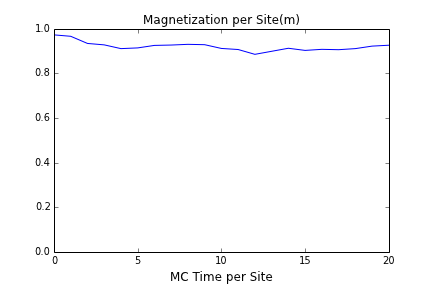
\includegraphics[width=\textwidth]
                {../../programs/graphics/equilibration_time/magnet_allup_T2,000000.png}
                \caption{All up initial spins corresponds to T=0}
        \end{subfigure}%
        ~ %add desired spacing between images, e. g. ~, \quad, \qquad etc.
          %(or a blank line to force the subfigure onto a new line)
        \begin{subfigure}[b]{0.5\textwidth}
                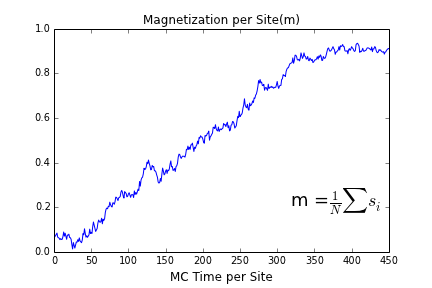
\includegraphics[width=\textwidth]
                {../../programs/graphics/equilibration_time/magnet_random_T2,000000.png}
                \caption{Random initial spins corresponds to T=$\infty$}
        \end{subfigure}
\end{figure}

\end{frame}\note{


Let's look at equilibration times at T=2.0. If we start simulation with all spins up, which corresponds to T=0 case, we will reach equilibrium after about 5 MC time per site. Also, if we start simulation with random spins which corresponds to T=$\infty$ case, we will reach equilibrium after about 350 MC time per site. Therefore, we can see that if our initial temperature, that we start the simulation, is close to our system’s temperature we will get equilibrium faster.

}

\subsection{Autocorrelation Function and Correlation Time}
\begin{frame}
\frametitle{Autocorrelation Function and Correlation Time}
Autocorrelation function for magnetization at T=2.0 is,
\begin{equation}
\chi (t) = \int dt' [m(t') - \langle m\rangle][m(t' + t) - \langle m\rangle] = \int dt'[m(t')m(t' + t) - {\langle m\rangle}^2]  
\end{equation}
\begin{figure}
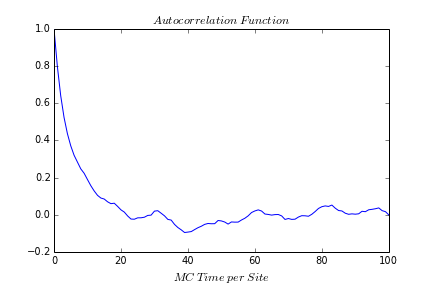
\includegraphics[scale=0.5]
 {../../programs/graphics/autocorrelation/autocorrelation2_T2,000000.png}
\end{figure}
\end{frame}
\note{

To find correlation time, we should look at autocorrelation function. 
Autocorrelation function gives correlation of two different values of 
magnetization with t time difference. We can see that if time between 
states is small, magnetizations are same and fluctuations are in the same 
direction. Hence, with summing them for all times, we get high positive 
autocorrelation value.  And if t is large, it means that we change a lot of 
spins between these 2 calculations, hence, magnetizations are different 
and fluctuations of magnetizations are different. Hence, autocorrelation is 
around 0. If autocorrelation function is not equal to 0 the fluctuations are 
correlated, on average.

// autocorrelation function acıklama. sadece 2 propertnin fluctuationları arasındaki correlation ı verir de. 

//Actually, autocorrelation is calculated by integrating over an infinite time. 
//ama yok infinite gibi yapmak için son magnetization degerlerini 
//bastakiler ile iliskilendirdik. bu yuzden sonlarda autocorrelation arttı 
//tekrar. 

}

\begin{frame}
Fitting autocorrelation function for early times,
\begin{equation}
\chi (t) \sim e^{-t/ \tau} \qquad log(\frac{\chi (\tau)}{\chi (0)}) = \frac{-t}{\tau}
\end{equation}
\begin{figure}
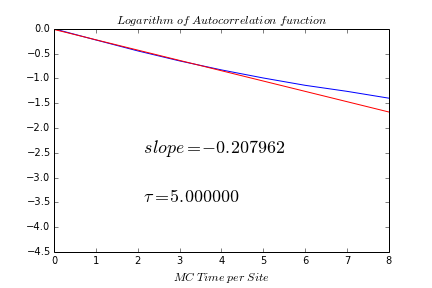
\includegraphics[scale=0.6] {../../programs/graphics/autocorrelation/correlation_fit_T2,000000.png}
\end{figure}
\end{frame}\note{

We know that autocorrelation is exponentially decaying function. Hence, if we normalize it, taking logarithm of it we can find correlation time by fitting a line. 

}

\begin{frame}
\frametitle{System Properties}
\begin{figure}
        \centering
        \begin{subfigure}[b]{0.5\textwidth}
        	\begin{equation}
	\langle m \rangle = \frac{1}{N} \left\langle \sum\limits_{i} s_i 
	\right\rangle
	\end{equation}
                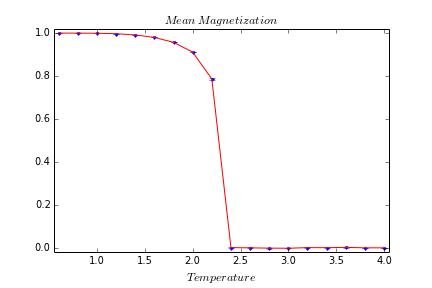
\includegraphics[width=\textwidth]
                {../../programs/graphics/properties/magnetization_L50.png}
                \caption{Mean magnetization per site vs Temperature}
        \end{subfigure}%
        ~ %add desired spacing between images, e. g. ~, \quad, \qquad etc.
          %(or a blank line to force the subfigure onto a new line)
        \begin{subfigure}[b]{0.5\textwidth}
        \begin{equation}
u = E_{ps} = \frac{1}{N} \langle \texttt{H} \rangle
	\end{equation}

                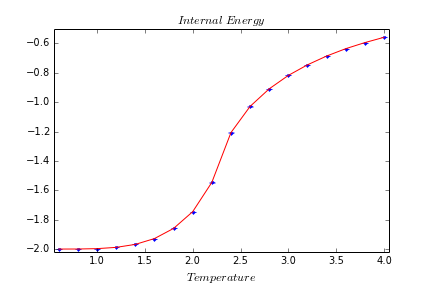
\includegraphics[width=\textwidth]
                 {../../programs/graphics/properties/internal_energy_L50.png}
                \caption{Internal energy per site vs Temperature}
        \end{subfigure}
\end{figure}
\end{frame}\note{
If we look at the plot, mean magnetization is 1 when T=0 and 0 when T=∞ 
as we expected. Also, if we increase the temperature from 0, we see that 
magnetization is about 1 until T is around 2.2. Also, if we keep on 
increasing the temperature, we will see a sharp decrease in magnetization 
to 0. This sharp change around when T is around 2.2 is called Phase 
Transition. 
Again, we see that a change in internal energy of the system when T is 
around 2.2. This is also caused by phase transition.

// direkt sharp olacaktı ama finite size. 

}

\begin{frame}
\begin{figure}
        \begin{subfigure}[b]{0.5\textwidth}
        \begin{gather}
\chi = \beta N [ \langle m^2 \rangle - \langle m \rangle^2    ]
\end{gather}
                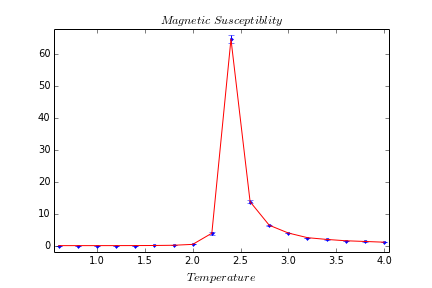
\includegraphics[width=\textwidth]
                {../../programs/graphics/properties/magnetic_suscept_L50.png}
                \caption{Magnetic suscept. vs Temperature}
        \end{subfigure}%
        ~ %add desired spacing between images, e. g. ~, \quad, \qquad etc.
          %(or a blank line to force the subfigure onto a new line)
        \begin{subfigure}[b]{0.5\textwidth}
        \begin{equation}
c = k \beta^2 N [ \langle E_{ps}^2 \rangle - \langle E_{ps} \rangle^2 ]
\end{equation}
                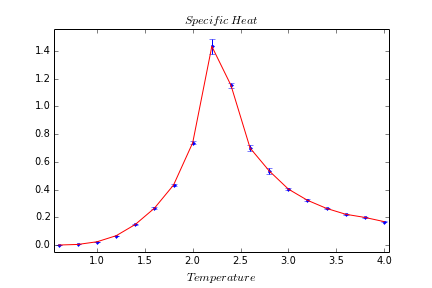
\includegraphics[width=\textwidth]
                 {../../programs/graphics/properties/specific_heat_L50.png}
                \caption{Specific heat vs Temperature}
        \end{subfigure}
\end{figure}
\end{frame}\note{
Let’s look at fluctuations in magnetization and energy, which are magnetic susceptibility and specific heat of the system.

We can see that fluctuations in the magnetization and energy is diverged at the temperature of phase transition. Hence, we see a peak at that temperature. Also, because of this increased fluctuations at the phase transition and increased correlation times at phase transition our error bars are increased

}

\begin{frame}
Look at correlation times:
\begin{figure}
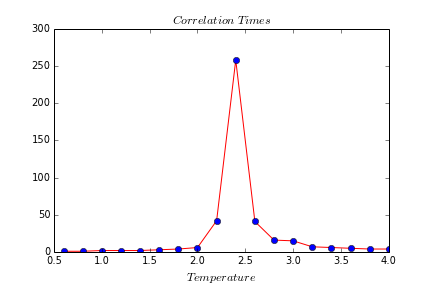
\includegraphics[scale=0.6]                  {../../programs/graphics/properties/correlation_time_L50.png}
                \caption{Correlation time vs Temperature}

\end{figure}
\end{frame}\note{

When phase transition occurs, our correlation times, states times between independent states, are diverged. Hence, because of that it is hard to simulate system around phase transition. Because, to get a lot of independent samples, we have to wait for a long time. Also, these increase in correlation time causes us to get a small number of independent samples; hence,causes increased error bars at the phase transition.

correlation time artar az veri ve fluctuationdan dolayı hata artar. 

}

\section{Investigation of System at Critical Temperature}
\subsection{Phase Transition and Critical Slowing Down}
\begin{frame}
Occurs at Critical temperature $T_c$. \\
For 2D Ising model, $T_c \approx 2.269$ \\
Property of Ising Model \\
Causes critical fluctuations \\
When we approach to phase transition correlation length increases. \\
Reduced temperature, $t$, is
\begin{equation}
t = \frac{T- T_c}{T_c}
\end{equation}
For Ising model, divergence of correlation length near phase transition goes like
\begin{equation}
\xi \propto |t|^{-\nu}
\end{equation}
$\nu$ is critical exponent.
Correlation Time per site 
\begin{equation}
\tau \propto |t|^{-z \nu} \propto \xi^{z}
\end{equation}
z is dynamic exponent.

\end{frame}\note{

Now, suppose we are at high temperatures where spins are random and 
uncorrelated. If we decrease temperature, interaction between spins forces 
spins to be in same direction. Hence, spins become correlated. Spin groups 
which are correlated because of these effect are called clusters and size of 
clusters are ξ, correlation length. This is because of the nature of the Ising 
model. 

Hence, when we flip a spin at critical temperature, these clusters will flip, 
because spins inside it are correlated, hence, we see fluctuations in 
magnetization and energy. and one of the error sources in 
critical region is these fluctuations.


When T is closer to critical temperature large regions of spins are in same 
direction. This regions are called 
domains. When T = Tc, there is about 3 percent chance to flip a spin inside 
a domain. Therefore, for Metropolis algorithm it is difficult to flip a spin 
because it tries to flip spin by spin. Because of that, correlation time is 
getting bigger at phase transition, this is called critical slowing down. Hence, other error source in critical region is correlation time. 

Hence, we can find a way to decrease correlation times to increase 
accuracy.

We define reduced temperature, absolute value of it gives how much we differ from phase transition. Also, for ising model, correlation length is in the form of (22). ν is critical exponent and is a property of Ising model
Hence, ξ depends only on nature of Ising model.

Also, we can define correlation time with using reduced temperature.  We konw that correlation time depends on our algorithm. and correlation time is defined as (23). Hence, z depends on our algorithm, then, we want small z values in our algorithm. z is dynamic exponent and (23) gives critical slowing down.

We can see that, if we reduce z with using another algorithm, we can reduce correlation time. 

}


\subsection{Wolff Algorithm}
\begin{frame}

\frametitle{Wolff Algorithm}

\begin{minipage}[t]{0.5\textwidth}
\begin{itemize}
\item Cluster-flipping algorithm \\
\item Look for clusters of similarly oriented spins and then flip them in their entirely all in one go, rather than trying to turn them over spin by spin. \\
\item To make a fair description of $\tau$
\begin{equation}
\tau = \tau_{steps} \frac{\langle n \rangle }{L^d}
\end{equation}
\end{itemize}
\end{minipage}\hfill
\begin{minipage}[t]{0.5\textwidth}
\begin{enumerate}
\item Select a spin randomly.
\item Look at the neighboring spins. If they are in same direction, add the cluster with probability $P_{add} = 1 - e^{-2 \beta J}$
\item For a spin that is added to the cluster, look at the neighboring spins of this spin and again add the spins with same direction which are not in the cluster with probability $P_{add}$
\item Repeat the process and complete the cluster
\item Flip the cluster
\end{enumerate}
\end{minipage}\hfill
\end{frame}\note{

In metropolis algorithm we flip only 1 spin and at critical temperature it is 
hard to flip a spin inside domain. But, chance of flip a spin at the edge of a 
domain is high because it has opposite spins in its neighbourhood, hence 
lower energy cost. The basic idea of Wolff algorithm is to look for clusters 
of similarly oriented spins and then flip them in their entirely all in one go, rather than trying to turn them over spin by spin. Hence, with using Cluster algorithms we can reduce critical slowing down.

// algoritmayı oku zaman kalırsa 

In Wolff algorithm we flip spins in a cluster. If there is n spins in a cluster, 
we flip n spins. Also, in Metropolis algorithm we flip 1 spin. Hence, to make 
a fair description of correlation time, this difference must be considered. 

To make a fair description of tau --> we can calculate correlation times in the form of eqn (24)

}

\subsection{Finite Size Scaling}
\begin{frame}
\frametitle{Finite Size Scaling}
\begin{equation}
\tau \propto L^{z}
\end{equation} 
\begin{figure}
        \centering
        \begin{subfigure}[b]{0.5\textwidth}
        
 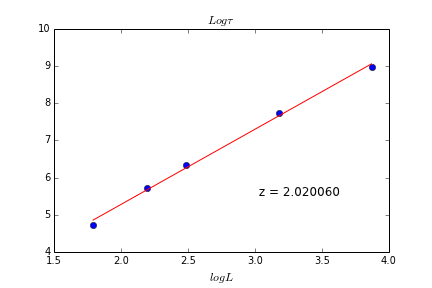
\includegraphics[scale=0.4]                  {../../programs/graphics/properties/dynamic_exponent.png}
                \caption{Metropolis Algorithm}
        \end{subfigure}%
        ~ %add desired spacing between images, e. g. ~, \quad, \qquad etc.
          %(or a blank line to force the subfigure onto a new line)
        \begin{subfigure}[b]{0.5\textwidth}
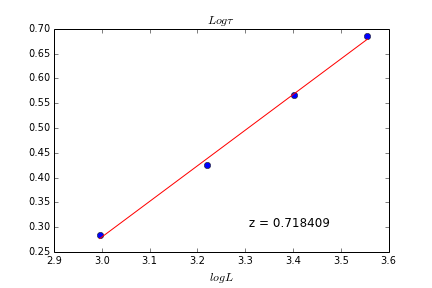
\includegraphics[scale=0.4]                  {../../programs/graphics/properties/dynamic_exponent_wolff.png}
                \caption{Wolff Algorithm}
        \end{subfigure}

\end{figure}

\end{frame}\note{

At T=Tc, cluster size diverges, but we are in a finite size system. Hence max. value of cluster size is L. Then correlation time is in the form of eq (25) at phase transition. 

We found that z = 2.02 for metropolis algorithm and z=0.72 for wolff algorithm. hence we can expect that correlation time can be decreased with using a cluster size algorithm. 
}



\end{document}











